\section{Auswertung}
	

	\subsection{Vertikalfeld}
		
		\noindent
				
		
	\subsection{Gyromagnetische Faktoren}
		
		\noindent
		Die Formel(\ref{eqn:zeeman}) lässt sich zu 
		\begin{equation}
			B = \frac{\hbar}{g_F \, \mu_B} \cdot \omega
			\label{eqn:steig}
		\end{equation}
		umstellen. In Abbildung(\ref{fig:Daten}) ist die Magnetfeldstärke gegen die RF-Frequenz gezeichnet.
		Hier lässt sich nun die Steigung der beiden Geraden mittels Gleichung(\ref{eqn:steig}) als $ m = \frac{\hbar}{g_F \, \mu_B}$ identifizieren.		
		Diese Steigung lässt sich wiederum zum gyromagnetischen Faktor
		\begin{equation}
		 	g_F = \frac{\hbar}{m \mu_B}
			\label{eqn:gyro}
		\end{equation}
		umstellen.		

		\begin{figure}[H]
			\centering
			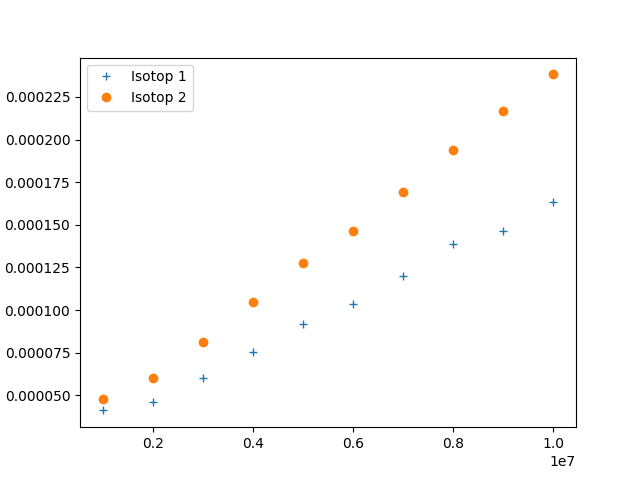
\includegraphics[width=0.7\textwidth]{build/Magnetfeld.png}
			\caption{Die gemessenen Daten geplotted mit den berechneten linearen Regressionen.}
			\label{fig:Daten} 
		\end{figure}

		\noindent
		Die Parameter der beiden Regressionen wurden zu:
		\begin{align}
			m_1 &= \SI{1.42(0.04)e-10}{\tesla\per\hertz}  &b_1= \SI{2.08(0.22)}{\tesla}\\
			m_2 &= \SI{2.17(0.04)e-10}{\tesla\per\hertz}  &b_2= \SI{1.92(0.23)}{\tesla}
		\end{align}
		bestimmt. Werden diese Steigungen nun in Gleichung(\ref{eqn:gyro}) eingesetzt, ergit sich für die die gyromagnetischen Faktoren:
		\begin{align}
			&\text{Isotop 1:} \quad g_\text{F} = \num{0.504(0.013)}\\
			&\text{Isotop 2:} \quad g_\text{F} = \num{0.329(0.006)}
		\end{align}

	\subsection{Kernspins}

	\subsection{Isotopenverhältnis}

	\subsection{Quadratischer Zeemann-Effekt}
